\documentclass[11pt]{article}
\usepackage[margin=1in]{geometry}
\usepackage{booktabs}
\usepackage{graphicx}
\usepackage{microtype}
\usepackage[hidelinks]{hyperref}

\newcommand{\structNet}{0.5}
\newcommand{\structTok}{6351}
\newcommand{\flatTok}{9380}
\newcommand{\winOverall}{4.906}
\newcommand{\winWtl}{7/1/0}
\newcommand{\extractedNet}{0.75}
\newcommand{\rolesNet}{0.25}
\newcommand{\aliasTok}{4862}


\title{\vspace{-2em}\textbf{Graph representation --- how the subgraph reaches the writer}}
\author{arxivkg · generation · graph representation}
\date{}

\begin{document}
\maketitle
\vspace{-2em}

\section*{What we did}
A retrieved citation subgraph (nodes, typed edges, non-linear) has to be serialized into a linear LLM
prompt. This is not a solved problem; each encoding has pros/cons. \textbf{Phase 1} compares the
\emph{structure} axis --- \texttt{flat\_list}, \texttt{adjacency\_list}, \texttt{dot} (Graphviz),
\texttt{subtree}, \texttt{json}, \texttt{matrix} --- judged absolute (4-axis) and order-debiased
pairwise vs \texttt{flat\_list}, over 8 deep-panel topics at T$=0$. \textbf{Phase 2} fixes the
adjacency winner and layers the \emph{orthogonal} axes: per-node \texttt{roles} (foundational/core/
frontier), per-node \texttt{extracted} content (full-text schema fields vs the abstract), and
\texttt{alias} (short \texttt{[D1]..} labels $+$ an id table).

\section*{Phase 1 --- structure}
\begin{center}\begin{tabular}{lrrr}
\toprule
representation & overall & pair\_net & tokens \\
\midrule
flat\_list & 4.312 & 0.0 & 9380 \\
\textbf{adjacency\_list} & 4.531 & 0.5 & 6351 \\
dot & 4.344 & 0.25 & 9211 \\
subtree & 4.344 & 0.375 & 8025 \\
json & 4.469 & 0.375 & 14476 \\
matrix & 4.438 & -0.125 & 7194 \\
\bottomrule
\end{tabular}
\end{center}
\begin{center}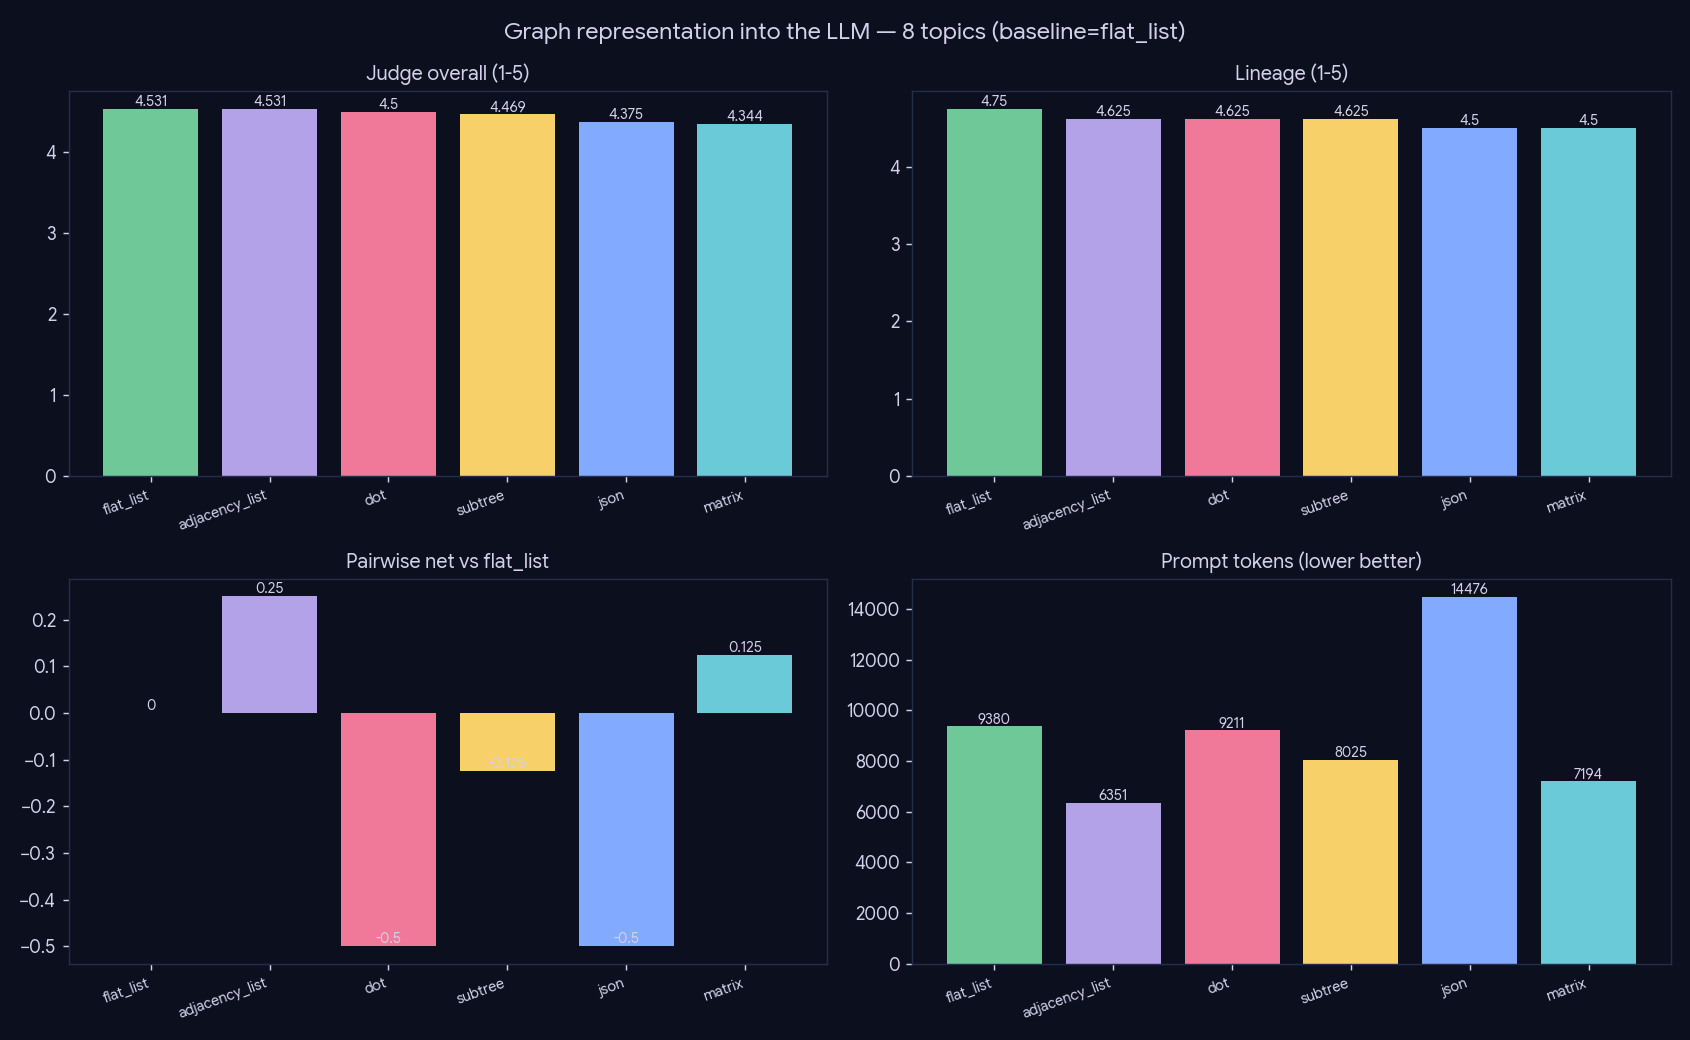
\includegraphics[width=0.9\textwidth]{../results/ablation.png}\end{center}

\section*{Phase 2 --- orthogonal axes on the adjacency winner}
\begin{center}\begin{tabular}{lrrrrr}
\toprule
config & cov. & lineage & overall & pair\_net & tokens \\
\midrule
flat\_list & 3.5 & 4.5 & 4.312 & 0.0 & 9380 \\
adjacency\_list & 3.75 & 4.625 & 4.531 & 0.5 & 6351 \\
adj\_roles & 4.125 & 3.875 & 4.438 & 0.25 & 6844 \\
adj\_extracted & 4.375 & 4.875 & 4.719 & 0.75 & 6690 \\
adj\_alias & 4.0 & 4.75 & 4.656 & 0.875 & 4862 \\
\textbf{adj\_roles\_extracted} & 4.625 & 5.0 & 4.906 & 0.875 & 6824 \\
\bottomrule
\end{tabular}
\end{center}
\begin{center}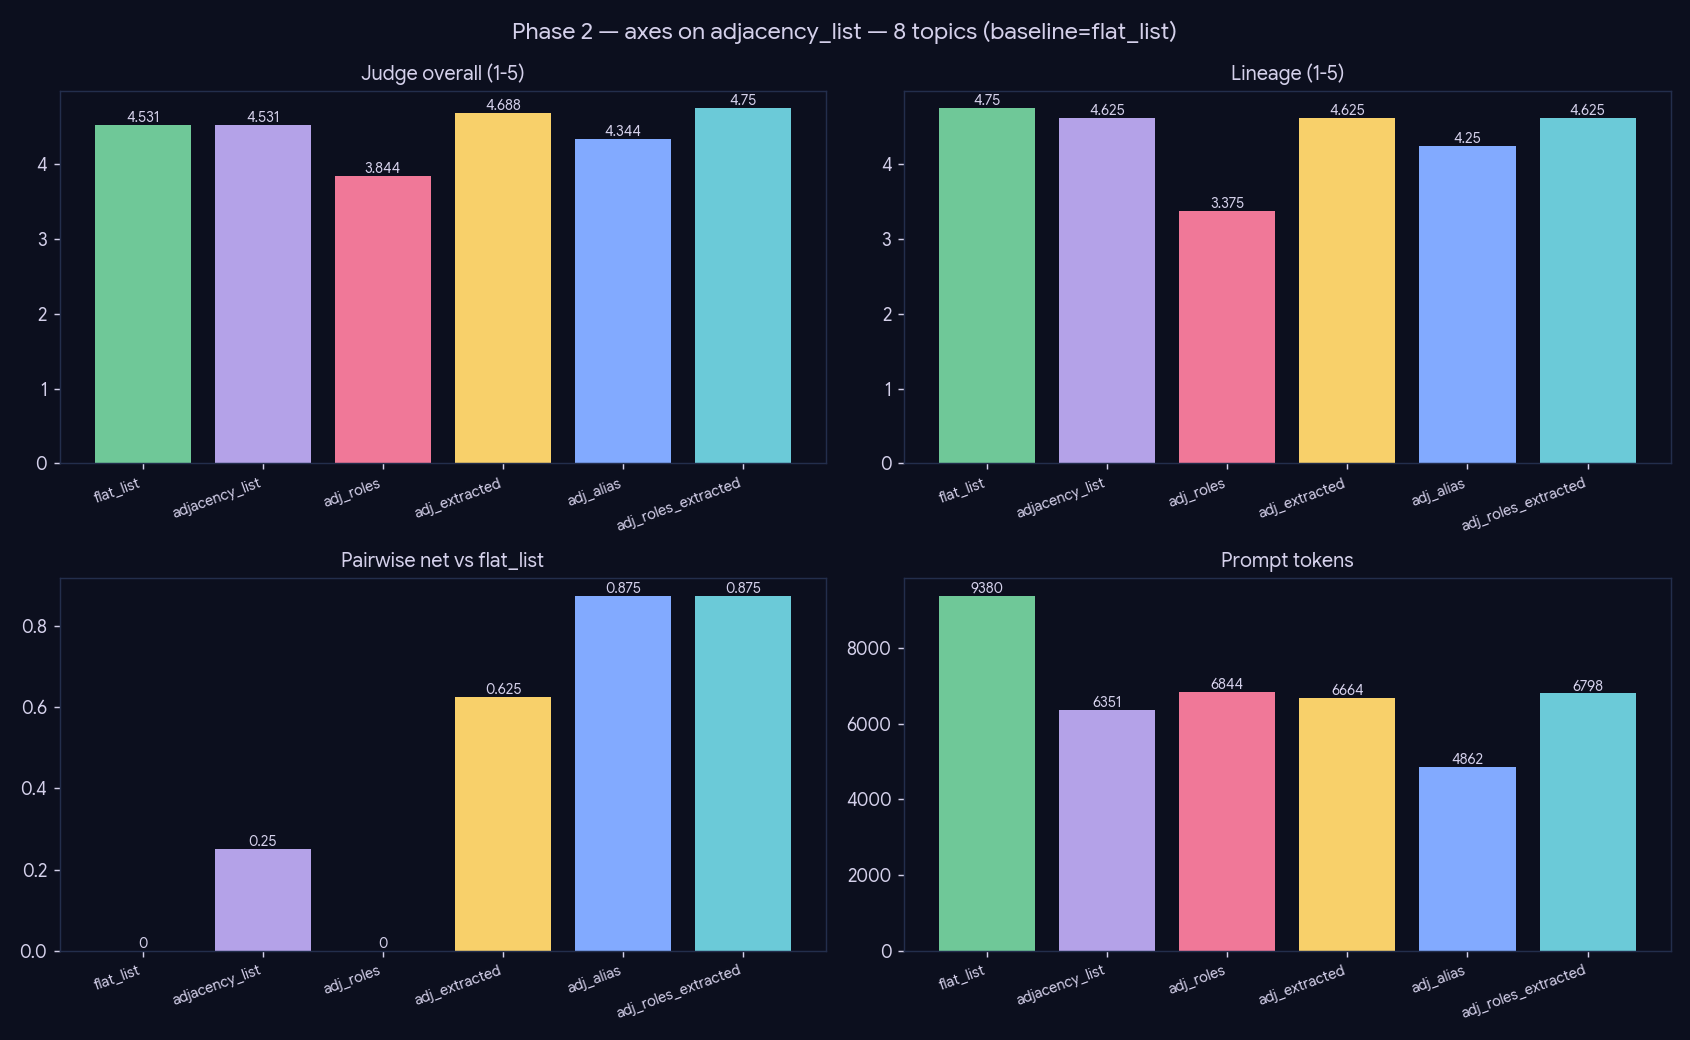
\includegraphics[width=0.9\textwidth]{../results/ablation_phase2.png}\end{center}

\section*{Conclusion}
\textbf{Structure: \texttt{adjacency\_list} wins} (pair\_net \structNet{}) --- and does it at the
\emph{fewest} tokens (\structTok{} vs \flatTok{} for flat, $2.3\times$ for json) --- a node table $+$
intent-grouped adjacency reads cleanly and compresses. \texttt{matrix} loses (negative net); \texttt{dot}/
\texttt{json} are middling and dearer. \textbf{Content is the biggest lever}: \texttt{adj\_extracted}
(full-text fields instead of abstracts) jumps to pair\_net \extractedNet{} --- specifics the abstract
omits are what the composer needs. \textbf{Roles help only \emph{with} content}: \texttt{adj\_roles}
alone is a weak \rolesNet{}, but combined the winner \texttt{adj\_roles\_extracted} tops every axis
(overall \winOverall{}, pairwise \winWtl{}). \textbf{Aliasing is a free token win}: \texttt{adj\_alias}
matches the top pairwise at the \emph{fewest} tokens (\aliasTok{}). \textbf{Production digest:
adjacency-list $+$ extracted content $+$ role tags $+$ aliasing.} \textbf{Caveat:} n$=8$, absolute axes
compressed; the pairwise nets are the discriminator and they agree across both phases.

\end{document}
